\documentclass[11pt,letterpaper]{article}
\usepackage[utf8]{inputenc}
\usepackage[T1]{fontenc}
\usepackage[spanish,es-nodecimaldot]{babel}
\usepackage{amsmath,amssymb,booktabs,float,graphicx,geometry,xcolor}
\usepackage{hyperref}
\usepackage{tikz}
\usetikzlibrary{arrows.meta,positioning}
\geometry{margin=2.5cm}
\graphicspath{{../figures/}}
\title{Clasificación de imágenes con tres modelos basados en VGG16}
\author{Nombre del estudiante}
\date{\today}

\newcommand{\arquitectura}[2]{%
\begin{figure}[H]\centering
\begin{tikzpicture}[node distance=5mm, every node/.style={font=\small,align=center}]
\node[draw,fill=blue!12,minimum width=2.2cm,minimum height=1.1cm] (in) {Entrada\\$224\times224\times3$};
\node[draw,fill=teal!25,right=of in,minimum width=3.2cm,minimum height=1.4cm] (vgg) {VGG16 convolucional\\congelada\\sin modificaciones};
\node[draw,fill=green!18,right=of vgg,minimum width=2.6cm,minimum height=1.1cm] (gap) {GlobalAveragePooling2D\\$7\times7\times512\to512$};
\node[draw,fill=orange!25,right=of gap,minimum width=3.2cm,minimum height=1.4cm] (head) {#2};
\draw[-{Latex}] (in)--(vgg); \draw[-{Latex}] (vgg)--(gap); \draw[-{Latex}] (gap)--(head);
\end{tikzpicture}
\caption{Arquitectura del Modelo #1. Únicamente cambia el cabezal naranja.}
\label{fig:arquitectura#1}
\end{figure}}

\begin{document}
\maketitle
\begin{abstract}
Se comparan tres clasificadores de flores que conservan intacta y congelada la
sección convolucional de VGG16. Los modelos difieren solamente en sus capas
densas. La comparación utiliza Accuracy, Precision, Recall y F1 Score sobre una
partición de prueba independiente.
\end{abstract}

\section{Conjunto de datos}
Se utiliza \texttt{tf\_flowers:3.0.1} de TensorFlow Datasets, compuesto por
3,670 imágenes RGB de cinco clases: dandelion, daisy, tulips, sunflowers y
roses \cite{tfdsflowers}. Como el catálogo ofrece un único split, se genera una
partición estratificada y determinista de 70\% entrenamiento, 15\% validación y
15\% prueba con semilla 42. Esta decisión conserva aproximadamente la
proporción de cada clase y evita emplear prueba para seleccionar el modelo.
Las imágenes tienen dimensiones y condiciones variables, por lo que se
redimensionan a $224\times224$ y se aplica \texttt{preprocess\_input} de VGG16.

\IfFileExists{../figures/histograma_clases_splits.png}{
\begin{figure}[H]\centering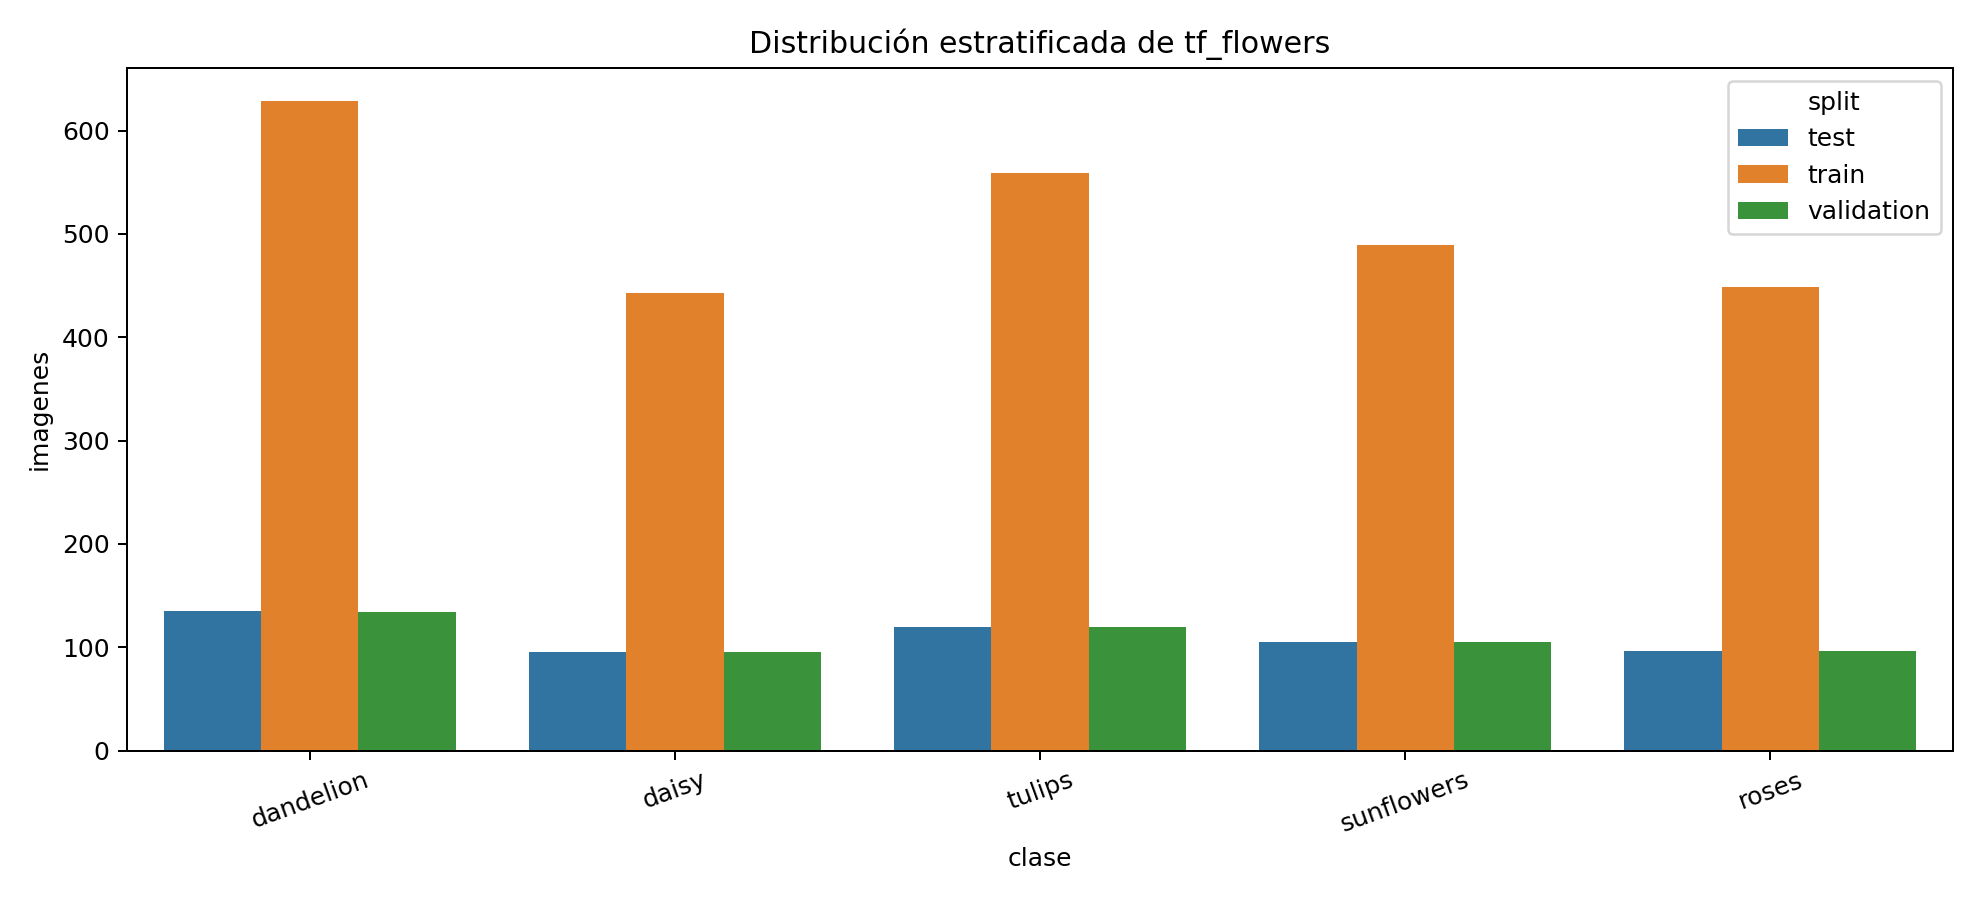
\includegraphics[width=.85\textwidth]{histograma_clases_splits.png}
\caption{Distribución por clase y partición.}\end{figure}}{}

\section{Metodología}
Los tres modelos emplean VGG16 preentrenada en ImageNet con
\texttt{include\_top=False}. Sus 13 capas convolucionales permanecen congeladas;
después se aplica \texttt{GlobalAveragePooling2D}. Todos usan Adam, tasa
$10^{-3}$, entropía cruzada categórica dispersa, lotes de 16, máximo 30 épocas,
early stopping y el mismo conjunto de datos aumentado.

\section{Modelos propuestos}
\arquitectura{A}{Dense 5\\Softmax}
El Modelo A es la línea base: sus cinco salidas aprenden una frontera lineal
sobre las 512 características, minimizando parámetros y riesgo de sobreajuste.

\arquitectura{B}{Dense 256, ReLU\\Dense 5, Softmax}
El Modelo B agrega 256 neuronas ReLU para aprender combinaciones no lineales
con una capacidad intermedia.

\arquitectura{C}{Dense 512, ReLU\\Dropout 0.5\\Dense 128, ReLU\\Dense 5, Softmax}
El Modelo C incrementa la capacidad y usa Dropout de 0.5 para reducir
coadaptación y controlar el sobreajuste en un dataset moderado.

\section{Métricas}
Para cada clase se interpreta el problema como uno-contra-el-resto:
\begin{align}
\mathrm{Accuracy}&=\frac{TP+TN}{TP+TN+FP+FN},&
\mathrm{Precision}&=\frac{TP}{TP+FP},\\
\mathrm{Recall}&=\frac{TP}{TP+FN},&
F_1&=2\frac{\mathrm{Precision}\,\mathrm{Recall}}
{\mathrm{Precision}+\mathrm{Recall}}.
\end{align}
Se presentan valores por clase y promedios macro y ponderado. F1 macro es el
criterio principal porque otorga el mismo peso a las cinco clases. Las filas de
la matriz de confusión son observaciones reales y las columnas predicciones.

\section{Resultados}
\IfFileExists{resultados_generados.tex}{\begin{table}[H]
\centering
\caption{Resultados sobre el conjunto de prueba.}
\label{tab:resultados}
\begin{tabular}{lrrrr}
\toprule
Modelo & Accuracy & Precision macro & Recall macro & F1 macro\\
\midrule
A & 0.8802 & 0.8798 & 0.8814 & 0.8799 \\
B & 0.8784 & 0.8785 & 0.8777 & 0.8775 \\
C & 0.8675 & 0.8713 & 0.8644 & 0.8652 \\
\bottomrule
\end{tabular}
\end{table}

\paragraph{Selección del mejor modelo.}
El Modelo A obtuvo el mayor F1 macro (0.8799), con Accuracy 0.8802. Por tanto, bajo la regla definida antes del experimento, es el modelo seleccionado. La interpretación por clase y los posibles indicios de sobreajuste deben contrastarse con las matrices de confusión y las curvas presentadas.

\paragraph{Análisis por clase.} En el modelo ganador, la clase con mayor F1 fue sunflowers (0.9048) y la de menor F1 fue roses (0.8317). La brecha absoluta entre F1 macro de validación y prueba fue 0.0219; este valor, junto con las curvas de aprendizaje, permite valorar la generalización sin basarse solamente en Accuracy.
}{
\textbf{Resultados pendientes de ejecución.} Ejecute los tres pares Train/Test
y después \texttt{python scripts/build\_report\_assets.py}.}

\foreach \m in {A,B,C}{%
\IfFileExists{../figures/arquitectura_modelo_\m.png}{
\begin{figure}[H]\centering
\includegraphics[width=.98\textwidth]{arquitectura_modelo_\m.png}
\caption{Diagrama exportado por el Train del Modelo \m.}\end{figure}}{}
\IfFileExists{../figures/curvas_modelo_\m.png}{
\begin{figure}[H]\centering
\includegraphics[width=.9\textwidth]{curvas_modelo_\m.png}
\caption{Curvas de entrenamiento y validación del Modelo \m.}\end{figure}}{}
\IfFileExists{../figures/matrices_confusion_modelo_\m.png}{
\begin{figure}[H]\centering
\includegraphics[width=.95\textwidth]{matrices_confusion_modelo_\m.png}
\caption{Matrices de confusión del Modelo \m.}\end{figure}}{}
\IfFileExists{../figures/metricas_clase_modelo_\m.png}{
\begin{figure}[H]\centering
\includegraphics[width=.85\textwidth]{metricas_clase_modelo_\m.png}
\caption{Precision, Recall y F1 por clase del Modelo \m.}\end{figure}}{}
\IfFileExists{../figures/histograma_confianza_modelo_\m.png}{
\begin{figure}[H]\centering
\includegraphics[width=.8\textwidth]{histograma_confianza_modelo_\m.png}
\caption{Histograma de confianza del Modelo \m.}\end{figure}}{}}

\IfFileExists{../figures/comparacion_modelos.png}{
\begin{figure}[H]\centering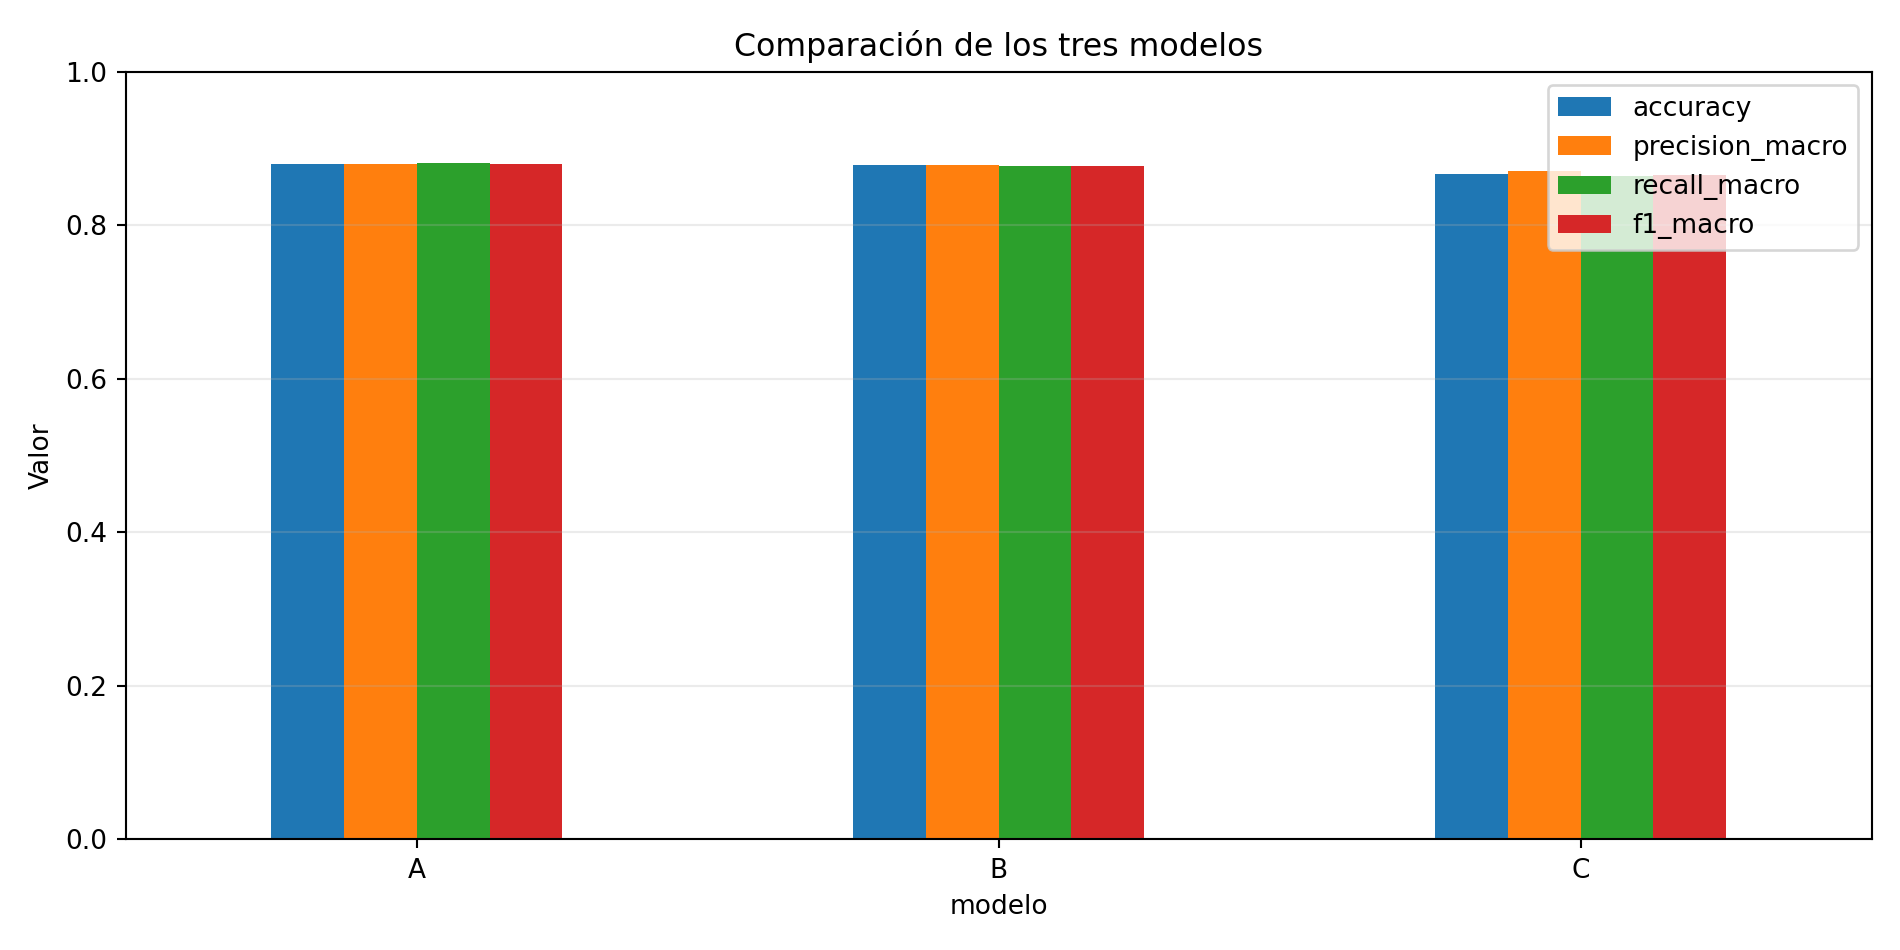
\includegraphics[width=.85\textwidth]{comparacion_modelos.png}
\caption{Comparación global de los tres modelos.}\end{figure}}{}

\section{Discusión}
Las curvas permiten contrastar convergencia y brecha entre entrenamiento y
validación; las matrices muestran qué pares de flores se confunden. Los
histogramas de confianza permiten detectar errores seguros, especialmente
relevantes al comparar mayor capacidad contra regularización. La discusión
final debe basarse en los archivos generados, no en valores estimados.

\section{Conclusión}
La selección sigue una regla fijada previamente: mayor F1 macro de prueba,
seguido por Accuracy y, si persiste el empate, menor complejidad. El texto
generado en la sección de resultados identifica al ganador únicamente después
de completar los tres experimentos.

\section{Reproducibilidad}
Se entregan seis notebooks Colab (Train y Test por modelo), configuración,
manifiesto de splits, historiales, predicciones, métricas, figuras, modelos
\texttt{.keras}, mejores pesos y hashes SHA-256. Cada Test carga exclusivamente
el modelo producido por su Train correspondiente.

\begin{thebibliography}{9}
\bibitem{tfdsflowers}
TensorFlow Team. \emph{tf\_flowers, TensorFlow Datasets Catalog}.
\url{https://www.tensorflow.org/datasets/catalog/tf_flowers}.
\bibitem{vgg}
K. Simonyan y A. Zisserman. \emph{Very Deep Convolutional Networks for
Large-Scale Image Recognition}, 2015.
\end{thebibliography}
\end{document}
